\section{Introduction}
\label{sec:intro}
Le présent rapport expose les travaux réalisés dans le cadre du cours Deep Learning II du Master Data Sciences de l'Institut Polytechnique de Paris. \\
L'étude porte sur la comparaison des performances en termes de précision de deux types de réseaux neuronaux: l'un pré-entraîné, l'autre initialisé de manière aléatoire. Les tests ont été effectués en modifiant différents paramètres, tels que le nombre de données d'apprentissage, le nombre de couches du réseau et le nombre de neurones par couche. 
Le but de l'étude était de classifier des images de chiffres manuscrits issus de la célèbre base de données MNIST.

\section{Étude sur Binary AlphaDigit}
Afin de vérifier la pertinence et la cohérence de nos programmes train\_RBM et train\_DBN que nous avons implémenté précédemment, nous allons nous concentrer sur l'étude exclusive de la base de données Binary AlphaDigit. Cette approche nous permettra de tester et de valider nos fonctions et notre approche. 

\subsection{Réseau Restricted Boltzmann Machines (RBM)}
Nous avons initié une série de tests non supervisés en utilisant un RBM avec les paramètres suivants:
\begin{itemize}
    \item Itération : 200
    \item Taux d'apprentissage : 0.1
    \item Taille des mini-batch : 32
\end{itemize}

Le modèle a été entraîné sur des données d'apprentissage appartenant à la classe du caractère '5', '6', 'H' et 'A'. Après entraînement du réseau RBM, la génération des images nous a donné le résultat suivant: 
\begin{figure}[H]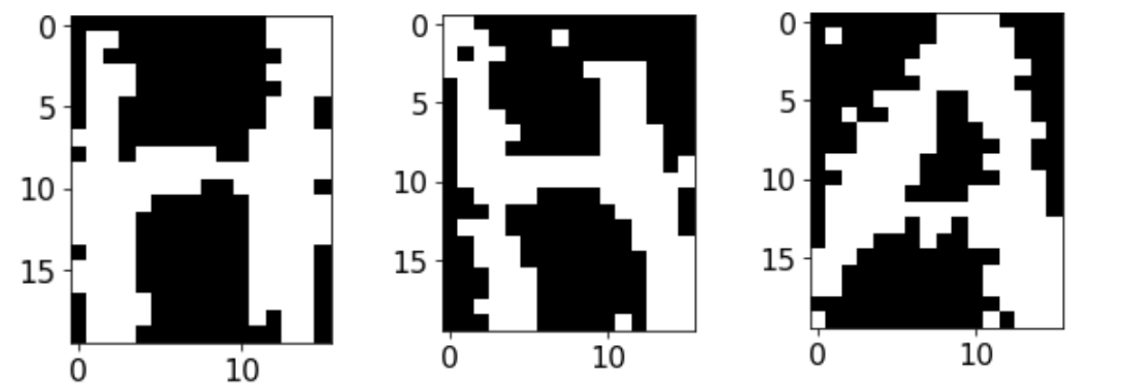
\includegraphics[width=140mm]{images/RBM.png}
\caption{génération de 3 images à l'aide du réseau RBM entraîné avec 4 chiffres}
\end{figure}

Il est évident que les images générées en sortie présentent une forte ressemblance avec les images d'entrée, tout en étant facilement identifiables et lisibles.

\subsection{Réseau Deep Belief Network (DBN)}
Nous allons reprendre les mêmes paramètres qui ont été utilisés pour l'entraînement du réseau RBM, que nous rappelons ci-dessous :
\begin{itemize}
    \item Itération : 200
    \item Taux d'apprentissage : 0.1
    \item Taille des mini-batch : 32
\end{itemize}
 
On obtient pour le DBN avec 3 couches et
200 neurones par couche:

\begin{figure}[H]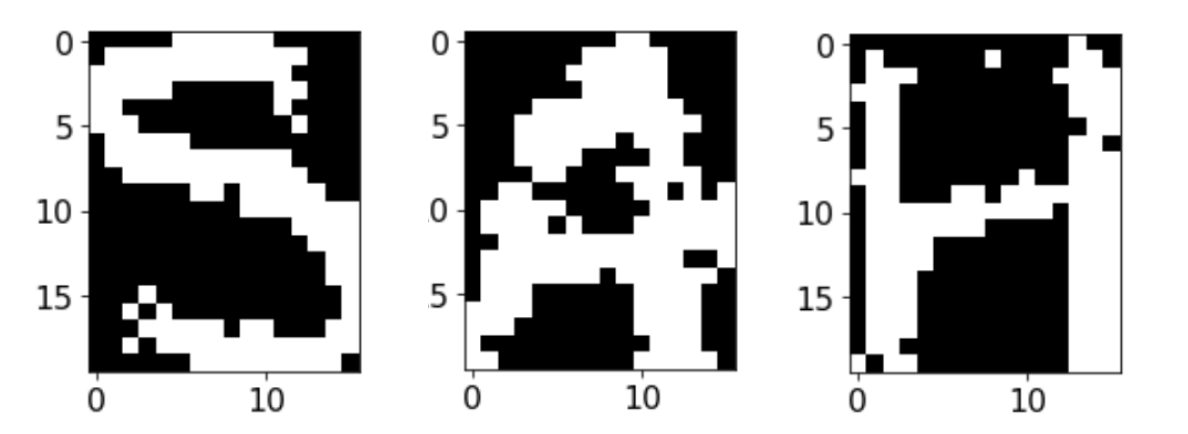
\includegraphics[width=140mm]{images/DBN.png}
\caption{génération de 3 images à l'aide du réseau DBN entraîné avec 4 chiffres}
\end{figure}

De manière générale, il est possible de constater que le DBN produit des images nettement plus lisibles que celles générées par le RBM.

En effet, les modèles génératifs tels que les RBM et DBN peuvent être limités en termes de la capacité à apprendre de nouveaux caractères, car ils nécessitent une grande quantité de données d'apprentissage pour capturer les variations subtiles entre les caractères. De plus, la complexité des modèles peut augmenter considérablement avec le nombre de caractères à apprendre, ce qui peut rendre l'apprentissage très lent et nécessiter des ressources informatiques importantes.
     
